\documentclass[12pt,a4paper]{article}
	%[fleqn] %%% --to make all equation left-algned--

% \usepackage[utf8]{inputenc}
% \DeclareUnicodeCharacter{1D12A}{\doublesharp}
% \DeclareUnicodeCharacter{2693}{\anchor}
% \usepackage{dingbat}
% \DeclareRobustCommand\dash\unskip\nobreak\thinspace{\textemdash\allowbreak\thinspace\ignorespaces}
\usepackage[top=2in, bottom=1in, left=1in, right=1in]{geometry}
%\usepackage{fullpage}

\usepackage{fancyhdr}\pagestyle{fancy}\rhead{Stephanie Wang}\lhead{EE236B homework 6}

\usepackage{amsmath,amssymb,amsthm,amsfonts,microtype,stmaryrd}
	%{mathtools,wasysym,yhmath}

\usepackage[usenames,dvipsnames]{xcolor}
\newcommand{\blue}[1]{\textcolor{blue}{#1}}
\newcommand{\red}[1]{\textcolor{red}{#1}}
\newcommand{\gray}[1]{\textcolor{gray}{#1}}
\newcommand{\fgreen}[1]{\textcolor{ForestGreen}{#1}}

\usepackage{mdframed}
	%\newtheorem{mdexample}{Example}
	\definecolor{warmgreen}{rgb}{0.8,0.9,0.85}
	% --Example:
	% \begin{center}
	% \begin{minipage}{0.7\textwidth}
	% \begin{mdframed}[backgroundcolor=warmgreen, 
	% skipabove=4pt,skipbelow=4pt,hidealllines=true, 
	% topline=false,leftline=false,middlelinewidth=10pt, 
	% roundcorner=10pt] 
	%%%% --CONTENTS-- %%%%
	% \end{mdframed}\end{minipage}\end{center}	

\usepackage{graphicx} \graphicspath{{}}
	% --Example:
	% \includegraphics[scale=0.5]{picture name}
%\usepackage{caption} %%% --some awful package to make caption...

\usepackage{hyperref}\hypersetup{linktocpage,colorlinks}\hypersetup{citecolor=black,filecolor=black,linkcolor=black,urlcolor=blue,breaklinks=true}

%%% --Text Fonts
%\usepackage{times} %%% --Times New Roman for LaTeX
%\usepackage{fontspec}\setmainfont{Times New Roman} %%% --Times New Roman; XeLaTeX only

%%% --Math Fonts
\renewcommand{\v}[1]{\ifmmode\mathbf{#1}\fi}
%\renewcommand{\mbf}[1]{\mathbf{#1}} %%% --vector
%\newcommand{\ca}[1]{\mathcal{#1}} %%% --"bigO"
%\newcommand{\bb}[1]{\mathbb{#1}} %%% --"Natural, Real numbers"
%\newcommand{\rom}[1]{\romannumeral{#1}} %%% --Roman numbers

%%% --Quick Arrows
\newcommand{\ra}[1]{\ifnum #1=1\rightarrow\fi\ifnum #1=2\Rightarrow\fi\ifnum #1=3\Rrightarrow\fi\ifnum #1=4\rightrightarrows\fi\ifnum #1=5\rightleftarrows\fi\ifnum #1=6\mapsto\fi\ifnum #1=7\iffalse\fi\fi\ifnum #1=8\twoheadrightarrow\fi\ifnum #1=9\rightharpoonup\fi\ifnum #1=0\rightharpoondown\fi}

%\newcommand{\la}[1]{\ifnum #1=1\leftarrow\fi\ifnum #1=2\Leftarrow\fi\ifnum #1=3\Lleftarrow\fi\ifnum #1=4\leftleftarrows\fi\ifnum #1=5\rightleftarrows\fi\ifnum #1=6\mapsfrom\ifnum #1=7\iffalse\fi\fi\ifnum #1=8\twoheadleftarrow\fi\ifnum #1=9\leftharpoonup\fi\ifnum #1=0\leftharpoondown\fi}

%\newcommand{\ua}[1]{\ifnum #1=1\uparrow\fi\ifnum #1=2\Uparrow\fi}
%\newcommand{\da}[1]{\ifnum #1=1\downarrow\fi\ifnum #1=2\Downarrow\fi}

%%% --Special Editor Config
\renewcommand{\ni}{\noindent}
\newcommand{\onum}[1]{\raisebox{.5pt}{\textcircled{\raisebox{-1pt} {#1}}}}

\newcommand{\claim}[1]{\underline{``{#1}":}}

\renewcommand{\l}{\left}\renewcommand{\r}{\right}

\newcommand{\casebrak}[4]{\left \{ \begin{array}{ll} {#1},&{#2}\\{#3},&{#4} \end{array} \right.}
%\newcommand{\ttm}[4]{\l[\begin{array}{cc}{#1}&{#2}\\{#3}&{#4}\end{array}\r]} %two-by-two-matrix
%\newcommand{\tv}[2]{\l[\begin{array}{c}{#1}\\{#2}\end{array}\r]}

\def\dps{\displaystyle}

\let\italiccorrection=\/
\def\/{\ifmmode\expandafter\frac\else\italiccorrection\fi}


%%% --General Math Symbols
\def\bc{\because}
\def\tf{\therefore}

%%% --Frequently used OPERATORS shorthand
\newcommand{\INT}[2]{\int_{#1}^{#2}}
% \newcommand{\UPINT}{\bar\int}
% \newcommand{\UPINTRd}{\overline{\int_{\bb R ^d}}}
\newcommand{\SUM}[2]{\sum\limits_{#1}^{#2}}
\newcommand{\PROD}[2]{\prod\limits_{#1}^{#2}}
\newcommand{\CUP}[2]{\bigcup\limits_{#1}^{#2}}
\newcommand{\CAP}[2]{\bigcap\limits_{#1}^{#2}}
% \newcommand{\SUP}[1]{\sup\limits_{#1}}
% \newcommand{\INF}[1]{\inf\limits_{#1}}
\DeclareMathOperator*{\argmin}{arg\,min}
\DeclareMathOperator*{\argmax}{arg\,max}
\newcommand{\pd}[2]{\frac{\partial{#1}}{\partial{#2}}}
\def\tr{\text{tr}}

\renewcommand{\o}{\circ}
\newcommand{\x}{\times}
\newcommand{\ox}{\otimes}

\newcommand\ie{{\it i.e. }}
\newcommand\wrt{{w.r.t. }}
\newcommand\dom{\mathbf{dom\:}}

%%% --Frequently used VARIABLES shorthand
\def\R{\ifmmode\mathbb R\fi}
\def\N{\ifmmode\mathbb N\fi}
\renewcommand{\O}{\mathcal{O}}

\newcommand{\dt}{\Delta t}
\def\vA{\mathbf{A}}
\def\vB{\mathbf{B}}\def\cB{\mathcal{B}}
\def\vC{\mathbf{C}}
\def\vD{\mathbf{D}}
\def\vE{\mathbf{E}}
\def\vF{\mathbf{F}}\def\tvF{\tilde{\mathbf{F}}}
\def\vG{\mathbf{G}}
\def\vH{\mathbf{H}}
\def\vI{\mathbf{I}}\def\cI{\mathcal{I}}
\def\vJ{\mathbf{J}}
\def\vK{\mathbf{K}}
\def\vL{\mathbf{L}}\def\cL{\mathcal{L}}
\def\vM{\mathbf{M}}
\def\vN{\mathbf{N}}\def\cN{\mathcal{N}}
\def\vO{\mathbf{O}}
\def\vP{\mathbf{P}}
\def\vQ{\mathbf{Q}}
\def\vR{\mathbf{R}}
\def\vS{\mathbf{S}}
\def\vT{\mathbf{T}}
\def\vU{\mathbf{U}}
\def\vV{\mathbf{V}}
\def\vW{\mathbf{W}}
\def\vX{\mathbf{X}}
\def\vY{\mathbf{Y}}
\def\vZ{\mathbf{Z}}

\def\va{\mathbf{a}}
\def\vb{\mathbf{b}}
\def\vc{\mathbf{c}}
\def\vd{\mathbf{d}}
\def\ve{\mathbf{e}}
\def\vf{\mathbf{f}}
\def\vg{\mathbf{g}}
\def\vh{\mathbf{h}}
\def\vi{\mathbf{i}}
\def\vj{\mathbf{j}}
\def\vk{\mathbf{k}}
\def\vl{\mathbf{l}}
\def\vm{\mathbf{m}}
\def\vn{\mathbf{n}}
\def\vo{\mathbf{o}}
\def\vp{\mathbf{p}}
\def\vq{\mathbf{q}}
\def\vr{\mathbf{r}}
\def\vs{\mathbf{s}}
\def\vt{\mathbf{t}}
\def\vu{\mathbf{u}}
\def\vv{\mathbf{v}}\def\tvv{\tilde{\mathbf{v}}}
\def\vw{\mathbf{w}}
\def\vx{\mathbf{x}}\def\tvx{\tilde{\mathbf{x}}}
\def\vy{\mathbf{y}}
\def\vz{\mathbf{z}}

%%% --Numerical analysis related
%\newcommand{\nxt}{^{n+1}}
%\newcommand{\pvs}{^{n-1}}
%\newcommand{\hfnxt}{^{n+\frac12}}

%%%%%%%%%%%%%%%%%%%%%%%%%%%%%%%%%%%%%%%%%%%%%%%%%%%%%%%%%%%%%%%%%%%%%%%%%%%%%%%%%%%%%%%%%%%%%%%%%%%%%%%%%%%%%%%%%%%%%%%%%%%%%%%%%%%%%%%%%%%%%%%%%%%%%%%%%%%%%%%%%%%%%%%%%%%%%%%%%%%%%%%%%%%%%%%%%%%%%%
\begin{document}
\subsubsection*{Additional Exercise 12.6 [Boyd \& Vandenberghe, 2017]}
{\it Ans:} (a) Assuming in the discretization $\theta^{tar}$ remains to be a node. Since $M \geq \max\{|G(\theta)| \mid |\theta_k - \theta^{tar}|\geq \Delta\}$ is equivalent to $M^2 \geq \max\{|G(\theta)|^2 \mid |\theta_k - \theta^{tar}|\geq \Delta\}$, we can write the SOCP
\begin{align*}
\mbox{minimize \;\;} & t\\
\mbox{subjected to \;\;} & G(\theta^{tar},\omega) = 1\\
& |G(\theta_k, \omega)|^2 \leq t \mbox{ for } k \mbox{ such that } |\theta_k - \theta^{tar}|\geq \Delta
\end{align*}
(b) The code associated with this problem is attached here. 
\begin{verbatim}
rand('state',0);
n = 40;
x = 30 * rand(1,n);
y = 30 * rand(1,n);

N = 400;
theta = linspace(-pi,pi,N)';
theta_tar = pi/12;
[~, tar_k] = min(abs(theta-theta_tar));
theta_tar_approx = theta(tar_k);
Delta = pi/12;
outside_index = (abs(theta-theta_tar)>= Delta);
G = @(omega) exp(1i*(cos(theta)*x+sin(theta)*y))*omega;
G_tar = @(omega) exp(1i*(cos(theta_tar_approx)*x+sin(theta_tar_approx)*y))*omega;

cvx_begin
    variable omega(n) complex
    variable t
    minimize t;
    subject to
        diag(outside_index)*abs(G(omega)) <= t*ones(N,1)
        G_tar(omega) == 1
cvx_end

h=semilogy(abs(G(omega)),'b-','LineWidth',1.2);
saveas(h, 'hw6P126','jpg');
\end{verbatim}
The graph of $|G(\theta)|$ with logarithm scaling is attached here.
\begin{center}
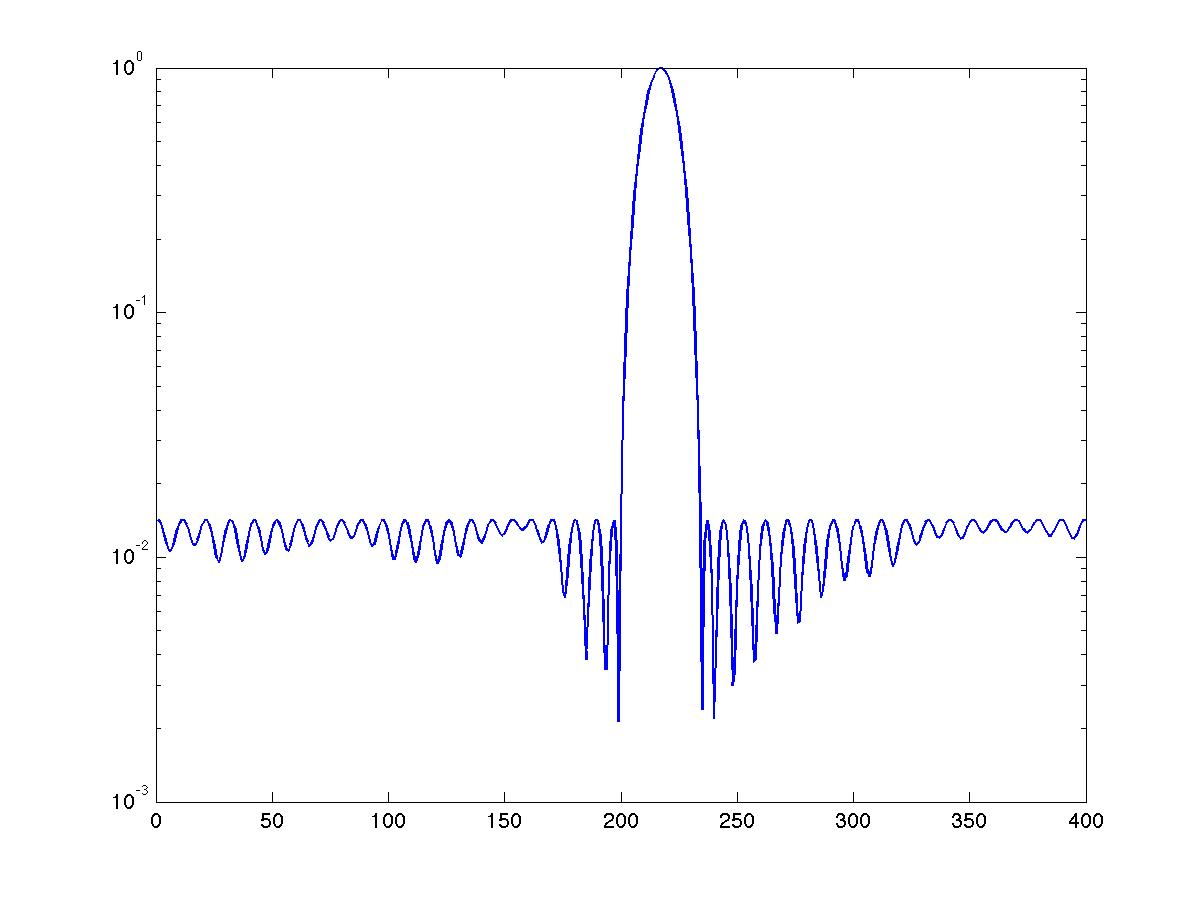
\includegraphics[scale=0.3]{hw6P126.jpg}
\end{center}





\newpage\subsubsection*{Additional Exercise 4.4 [Boyd \& Vandenberghe, 2017]}
{\it Ans:} The KKT condition to the problem is \onum1 $x^Tx - t = 0$, \onum2 (No inequality constraint. Skipped.), \onum3 (No inequality constraint. Skipped.), \onum4 the vanishing gradient (w.r.t. $x$ and $t$) of Lagrangian,
$$\SUM{k=1}m -4\l(t-2y_k^T x + \|y_k\|_2^2 - d_k^2\r)y_k + 2\nu x= 0$$
$$\SUM{k=1}m 2\l(t-2y_k^T x + \|y_k\|_2^2 - d_k^2\r)  - \nu= 0$$
Rearrange the above two equations we can solve for $x$ and $t$ once $\nu$ is given. The Lagrangian dual function is 
\begin{align*}
g(\nu) &= \inf_{x, t} \l(\SUM{k=1}m \l(t-2y_k^Tx + \|y_k\|_2^2 - d_k^2\r)^2 + \nu(x^Tx - t)\r) \\
&= \inf_{x, t} \l(\SUM{k=1}m \l(\|x-y_k\|_2^2 - d_k^2 - x^Tx + t \r)^2 + \nu(x^Tx - t)\r)
\end{align*}


\newpage\subsubsection*{Exercise 4.43 (b, c) [Boyd \& Vandenberghe, 2004]}
{\it Ans:} (b) Note that the smallest eigenvalue $\lambda_m(x) = \lambda_{min}(A(x))$ also has a similar relation
$$\lambda_{min}(A) \geq s \Longleftrightarrow A \succeq sI$$
Therefore the problem can be formulated as 
\begin{align*}
\mbox{minimize \;\;} & t - s\\
\mbox{subjected to \;\;} & A(x) \preceq tI \\
& sI \preceq A(x)
\end{align*}
(c) We need to do the problem
\begin{align*}
\mbox{minimize \;\;} & \lambda / \gamma\\
\mbox{subjected to \;\;} & A(x) \preceq \lambda I \\
& \gamma I \preceq A(x) \\
& 0 \prec \gamma I
\end{align*}
Following the hint to change the variable, $y = \/x\gamma, t = \/\lambda\gamma, s = \/1\gamma$, then $A(x) = A_0 + x_1 A_1 + \cdots + x_n A_n = \gamma(sA_0 + y_1 A_1 + \cdots + y_nA_n )$, and the problem becomes
\begin{align*}
\mbox{minimize \;\;} & t \\
\mbox{subjected to \;\;} & sA_0 + y_1A_1 + \cdots + y_nA_n \preceq t I \\
&  I \preceq sA_0 + y_1A_1 + \cdots +  y_nA_n
\end{align*}\qed




\newpage\subsubsection*{Exercise 5.19 [Boyd \& Vandenberghe, 2004]}
{\it Ans:} (a) The optimal value is 
$$\max \l\{ \SUM{i=1}n y_ix_i \mid y_i \in [0,1], \SUM{i=1}n y_i = r\r\}$$
Since this is linear in $x$, the optimal value can only be lumping the weights ($y_i$'s) on the largest $r$ components of $x$.  \\
(b) The Lagrangian dual function is (note the original problem is maximizing $x^T y$, so I translated it to minimizing $-x^T y$.)
\begin{align*}
g(\lambda_1, \lambda_2, \nu; x) &= \inf_y -x^Ty -\lambda_1^Ty + \lambda_2^T(y - \mathbf 1) + \nu (\mathbf 1^Ty - r) \\
&= \inf_y  y^T(-x -\lambda_1 + \lambda_2 + \nu \mathbf 1) - \mathbf1^T \lambda_2 - \nu r \\
&= \casebrak{ -\mathbf1^T\lambda_2 - \nu r}{-x-\lambda_1+\lambda_2 + \nu\mathbf1 = 0}{\-\infty}{\mbox{else}}
\end{align*}
The dual problem is then
\begin{align*}
\mbox{maximize \;\;} & -\mathbf1^T\lambda_2 - \nu r\\
\mbox{subjected to \;\;} & -x-\lambda_1+\lambda_2 + \nu\mathbf1 = 0 \\
&  \lambda_1 \succeq 0\\
& \lambda_2 \succeq 0
\end{align*}
Or if we let $\lambda_2 = u, \nu = t$ and combine the two constraints of $\lambda_1$, 
\begin{align*}
\mbox{maximize \;\;} & -\mathbf1^Tu - tr\\
\mbox{subjected to \;\;} & -x+u + t\mathbf1 \succeq 0 \\
& u \succeq 0
\end{align*}
This is essentially the same as given in the problem. The three conditions $rt + \mathbf1^Tu\leq \alpha, t\mathbf1 + u \succeq x, u\succeq 0$ just mean that the optimal value of the dual LP (which is the same as the primal LP, which is $f(x)$) is less than or equal to $\alpha$. \\
\\
(c) Here the constraint $\SUM{i=1}{\lfloor0.1n\rfloor} x_{[i]} \leq 0.8$ yields $r = \lfloor0.1n\rfloor, \alpha = 0.8$; that is, the problem can be formulated using the technique discussed above as 
\begin{align*}
\mbox{minimize \;\;} & x^T\Sigma x\\
\mbox{subjected to \;\;} & \bar p^T x \geq r_{min} \\
& \mathbf1^T x = 1\\
& x\succeq 0\\
&  \lfloor0.1n\rfloor t + \mathbf1^Tu \leq 0.8\\
& t\mathbf1 + u \succeq x\\
& u \succeq 0 \\
\end{align*}
with variables $x \in \R^n, t\in\R, u\in\R^n$. \qed





\newpage\subsubsection*{Exercise 5.21 (a, b, c) [Boyd \& Vandenberghe, 2004]}
{\it Ans:} (a) For sure $\/{d^2}{dx^2} e^{-x} = (-1)^2 e^{-x} = e^{-x} > 0$, the cost function is convex. Let $f_1(x, y) = x^2/y$. 
\begin{align*}
\nabla f_1(x, y) &= \l[\begin{array}{cc}2x/y& -x^2/y^2\end{array}\r]\\
H_{f_1}(x, y) &= \displaystyle\l[\begin{array}{cc}
\frac2y & \frac{-2x}{y^2} \\
\frac{-2x}{y^2} & \frac{2x^2}{y^3}
\end{array}\r] 
\end{align*}
and $H_{f_1}(x, y)\succeq 0$ since $\/2y >0$ and $\det(H_{f_1}(x, y)) = \/{4x^2}{y^4} - \/{4x^2}{y^4} = 0 \geq 0$. The constraint function is essentially ruling $x = 0$ since the domain $\mathcal D$ restricts $y > 0$; with this observation, we conclude the optimal value to the problem is $e^{-0} = 1$. \\
\\
(b) First observe the Lagrangian is always positive for nonnegative $\lambda$, 
$$L(x, y, \lambda) =  e^{-x} + \lambda \frac{x^2}y \geq 0$$
since $e^{-x} > 0$ and $x^2 / y \geq 0$. Now consider $y = \lambda x^4$ as $x\ra1 \infty$, then 
$$L(x, y, \lambda, \nu) =  e^{-x} + \lambda \frac{x^2}y = e^{-x} + \/{1}{x^2} \ra1 0$$
That is, the Lagrangian dual function
$$g(\lambda) = \inf_{x, y} L(x, y, \lambda) = 0$$
is the zero constant function regardless of the input $\lambda$. Hence any $\lambda \geq 0$ can be optimal solution to the dual problem
\begin{align*}
\mbox{minimize \;\;} & g(\lambda)\\
\mbox{subjected to \;\;} & \lambda \geq 0\end{align*}
and the optimal value $d^\ast = 0$. Notice a optimal duality gap $p^\ast - d^\ast =  1 - 0 = 1$. \\
\\
(c) Note that the Slater's condition does not hold for this problem since there exists no $x$ and $y$ such that $x^2/y < 0$ and $y>0$. \qed


\newpage\subsubsection*{Additional Exercise 4.30 [Boyd \& Vandenberghe, 2017]}
{\it Ans:} (a) The Lagrangian dual function is
\begin{align*}
g(\lambda) &= \inf_{x, y}\l( c^T x + \frac1\mu \SUM{i=1}m \log(1+e^{\mu y_i}) + \lambda^T (Ax-b-y)\r) \\
&= - \lambda^T b + \inf_{x, y} \l(  x^T(c+A^T\lambda) + \frac1\mu \SUM{i=1}m \log(1+e^{\mu y_i}) -\lambda^T y\r) 
\end{align*}
The $y$ part is minimized when
$$\frac1\mu \cdot \frac{\mu e^{\mu y_i}}{1+e^{\mu y_i}} - \lambda_i = 0 \mbox{ for }i = 1, \cdots, m$$
or 
$$y_i = \frac1\mu \log\l(\frac{\lambda_i}{1-\lambda_i}\r) \mbox{ for } i = 1, \cdots m$$
therefore, 
\begin{align*}
g(\lambda) &= - \lambda^T b + \inf_{x, y} \l( x^T(c+A^T\lambda) + \frac1\mu \SUM{i=1}m \log(1+e^{\mu y_i}) -\lambda^T y  \r)\\
&= -\lambda^Tb + \frac1\mu \SUM{i=1}m \log\l(\frac1{1-\lambda}\r) - \SUM{i=1}m \frac{\lambda_i}{\mu} \log\l(\frac{\lambda_i}{1-\lambda_i}\r) + \inf_x x^T(c+A^T\lambda)\\
&= -\lambda^Tb-\frac{1}\mu\SUM{i=1}m \l((1-\lambda_i)\log(1-\lambda_i) + \lambda_i\log(\lambda)\r) + \inf_x x^T(c+A^T\lambda) \\
& =\casebrak{-b^T\lambda + \frac1\mu\SUM{i=1}m \log\l(\lambda_i^{\lambda_i}(1-\lambda_i)^{1-\lambda_i}\r)}{c+A^T\lambda = 0}{-\infty}{\mbox{else}}
\end{align*}
with the domain restriction that $\lambda_i \in (0,1)$ for $i=1, \cdots, m$. \\
\\
(b) (Note I used $\lambda$ as my dual variable where it's $z$ in the problem.) The Lagrangian dual of the dual linear program is 
$$\tilde g(z) = \casebrak{-b^Tz}{A^Tz+c = 0}{-\infty}{\mbox{else}}$$
Assuming strong duality (assume so because the linear program and its dual has it), the optimal value of problem (25) is $q^\ast = g(\lambda^\ast)$ for some $\lambda^\ast$. Now since $z^\ast$ is an optimal solution to the dual linear program, we see it provides an upper bound
$$q^\ast \leq g(z^\ast) = -b^Tz^\ast + \frac1\mu\SUM{i=1}m \log\l({z_i^\ast}^{z_i^\ast}(1-z_i^\ast)^{1-z^\ast_i}\r) \leq p^\ast + \frac1\mu\SUM{i=1}m\log2$$
the last inequality follows from that $0\preceq z^\ast \preceq \mathbf1$.
The other side of the inequality required is not much but from the fact that $p^\ast \leq g(\lambda)$ whenever $g(\lambda)$ is defined. \qed





\end{document}
